\section{Modelando contextos arm\'onicos}
\label{sec:harmonic_contexts}
\subsection{Contextos}
Una car'acteristica de la m'usica compartida con el habla es que un mismo s'imbolo es interpretado de distinta forma seg'un el contexto
en donde este sea percibido. En el caso del habla, se refiere por s'imbolo a una palabra. Esta diferencia interpretativa es conocida 
como polisemia, y refiere a la cualidad de una palabra de tener m'as de un significado. Por ejemplo, la palabra \emph{sierra}, refiere
tanto a un instrumento que permite cortar madera, como a una parte de la cordillera. De esta forma, en la oraci'on 
``Lindo viaje por la sierra'' atribuye un significado a la palabra sierra, mientras que ``Compr'e una sierra nueva, puesto que la vieja 
estaba gastada'' atribuye el otro significado. 

Este mismo fen'omeno ocurre con la m'usica, lo que cambia es la noci'on de \emph{contexto} y de \emph{interpretaci'on}. En este caso
la interpretaci'on estar'a relacionada con el \emph{grado de de estabilidad} que genera una cierta nota, y el contexto estar'a dado por
una pieza musical; una nota por si sola no es ni estable ni inestable, lo es en un cierto \emph{contexto}. Si bien es cierto que a una nota
se le atribuye un grado de estabilidad en el contexto de una pieza, esta definici'on es por dem'as vaga. A continuaci'on se refinar'a
este concepto.

Carol Krumhansl \citep{Krumhansl90} refiere a estas relaciones de estabilidad como jer'arquicas, en el sentido de que existen elementos normativos que son tomados 
como punto de referencia. Este fen'omeno no es exclusivo de la m'usica; los colores son frecuentemente descriptos respecto a ciertos colores 
focales como rojo, verde, azul, y amarillo. Los n'umeros son comparados con otros que tienen un status cognitivo especial: 9 es casi 10, 95 es casi 100. 
De esta forma, se refiere a las relaciones entre las alturas como \texttt{la jerarqu'ia tonal}. Basada en estos principios, Krumhansl, 
propone m'etodos emp'iricos para cuantificar esta jerarqu'ia.

%Karol Krumhansl refiere en \cita a la m'usica occidental como tonal-arm'onica, haciendo referencia a dos propiedades importantes que rigen
%su coherencia. Por tonal, se refiere a el hecho de que las piezas musicales occidentales est'an organizadas al rededor de una cierta 
%nota denominada \emph{t'onica}, a su vez, por harm'onica se refiere al marco para establecer las relaciones entre las alturas respecto a la t'onica. Krumhansl contin'ua
%identificando tres elementos dentro de la musica tonal-arm'onica: alturas, acordes y tonalidades.

%Por altura se refiere a una de las posible 12 categor'ias disponibles en la m'usica tonal, por acorde, a cualquier grupo de 3 o m'as 
%notas que suenen en simult'aneo\footnote{esa es la definici'on que esta en la pagina 9\ldots no habla de superposici'on de 3ras}, y por 
%tonalidad a la t'onica y su escala, que es un patr'on de intervalos definidos en relaci'on a la t'onica. 

Fred Lerdahl \citep{Lerdahl2001} en su libro A Tonal Pitch Space contin'ua en cierto grado con el trabajo de Krumhansl, y define un espacio en donde pretende 
modelar, entre otras cosas, el grado de estabilidad de una nota en un cierto contexto, definiendo contexto a partir de dos cosas: una tonalidad y un acorde. 
El libro es mucho m'as general y abarcativo que lo reci'en mencionado, pero a los efectos de este trabajo, s'olo se tomar'a esa parte.

En lo que sigue, se presenta con mayor detalle parte de los estudios de Krumhansl y Lerdahl, para luego dar un marco bayesiano sobre el cual montar las jerarqu'ias tonales.

\subsection{Pitch profiles}
A continuaci'on se describir'a el m'etodo propuesto por Krumhansl para cuantificar la jerarqu'ia tonal, y su aplicaci'on para cuantificar el grado de estabilidad 
de una nota en dicha jerarqu'ia. 
El m'etodo es llamado \emph{probe tone method} y se basa en el siguiente hecho: Krumhansl observ'o en sus experimentos que cuando se presentaba a un sujeto una escala 
incompleta, esta genera una fuerte expectativa sobre el tono faltante. Por ejemplo, si sonaran las notas C, D, E, F, G, A, B en ese orden, se generar'ia una fuerte 
expectativa de escuchar C, y no s'olo esto, sino que este fen'omeno es independiente de la octava en la que se produzca el C para completar.
Krumhansl denomina a esta 'ultima nota \emph{probe tone}, y su experimento se basa en exponer al oyente a todas las posibles continuaciones, y que este de un puntaje
seg'un cuan buena considera la continuaci'on escuchada. Una vez presentadas todas las continuaciones para la escala con el C faltante, se rota la escala, y se procede
de la misma forma con D. De esta forma, el experimento con D constar'ia en presentar al sujeto la siguiente sucecion de notas: D, E, F, G, A, B, C, para luego pedir
que califique las continuaciones, esperando que la mejor continuaci'on sea D.

Una vez finalizado el experimento, la informaci'on se recopila para construir el pitch profile. \alert{como cornos se construye?}

El experimento se realiz'o tanto con sujetos con y sin entrenamiento musical. Si bien el nivel de ruido aumenta a medida que los sujetos 
tienen menor entrenamiento musical, las tendencias permanecen. En la figura \ref{fig:pitch_profile} se exhibe un ejemplo de pitch profile para la escala mayor: 
el eje X representa todas las alturas dentro de una escala, el eje Y simboliza el grado de estabilidad. De esta forma, se puede observar que los grados arm'onicos
1, 3 y 5 (C, E y G en la escala de C mayor) son los m'as estables, luego le sigue los tonos correspondientes el resto de la escala mayor, y por 'ultimo el resto de los 
tonos.


\begin{imagen}
    \file{images/pitch_profile.png}
    \labelname{fig:pitch_profile}
    \desc{El pitch profile para m'usicos}
    \width{10cm}
\end{imagen}


En su trabajo, Krumhansl propone distintas caracter'isticas, y las analiza mediante t'ecnicas de regresi'on, llegando a la conclusi'on que la
caracter'istica m'as importante es la duraci'on relativa de una nota respecto al resto: La nota cuya proporci\'on es mayor en el tema ser'a la t'onica. A partir de este 
estudio, es posible entonces inferir un pitch profile. Dado que a los efectos de generar una melod'ia no es de inter'es saber el nombre de la tonalidad, se propone 
utilizar el pitch profile como distribuci'on de probabilidades para la elecci'on de las notas.

\subsection{El espacio diat\'onico}
Hist'oricamente se han hecho una gran cantidad de intentos por encuadrar dentro de un modelo grafico/espacial las relaciones de estabilidad entre elementos de la m'usica
tonal. Ejemplos son el c'irculo de quintas y de terceras \alert{poner dibujos}. Fred Lerdahl \citep{Lerdahl2001} propone un espacio para distintas entidades tonales como alturas, 
acordes y tonalidades. En 'el, define una noci'on de distancia que pretende reflejar el parentezco entre las entidades en t'erminos de estabilidad, es decir, no solo 
mide la estabilidad de una nota dentro de un contexto, sino que tambi'en mide la distancia entre dos acordes dentro de una tonalidad, y la distancia entre dos tonalidades. 
Nuevamente, no es de inter'es medir esas distancias, sin embargo, se considera que el comportamiento que tiene el modelo de Lerdahl es deseable en un modelo estad'istico
que vaya a cuantificar la estabilidad de una nota.

El autor trabaja con la noci'on de contexto como una mezcla entre la tonalidad que rige en el tema (o en esa parte, ver secci'on \ref{sec:musical_intro}) y el
acorde que gobierna la estabilidad en ese momento. El primero lo denomina como \emph{espacio b'asico}\alert{no existe una traducci'on linda?}. 
El espacio b'asico refleja las relaciones de estabilidad que les son aplicadas a las notas en relacion a una tonalidad. 

En la figura \ref{fig:basic_space} se exhibe una representaci'on gr'afica del espacio tonal b'asico para la tonalidad de Do mayor. En el eje vertical, se encuentra
representado el nivel de estabilidad: Una nota que esta en el nivel \texttt{a} ser'a m'as estable que una nota que se encuentre en un nivel inferior. Como 
podr'a verse, todas las notas se encuentran en el nivel \texttt{e}, de menor estabilidad, y a medida que se sube de nivel, s'olo un subconjunto de notas son las 
que persisten, sin embargo, notas de niveles superiores siembre tienen su lugar en los niveles inferiores.

\begin{center}
\begin{tabular}{r c c c c c c c c c c c c c} 
\label{fig:basic_space}
a) & C &     &   &     &   &   &     &   &     &   &     &   & C\\
b) & C &     &   &     &   &   &     & G &     &   &     &   & C\\
c) & C &     &   &     & E &   &     & G &     &   &     &   & C\\
d) & C &     & D &     & E & F &     & G &     & A &     & B & C\\
e) & C & C\# & D & D\# & E & F & F\# & G & G\# & A & A\# & B & C\\
\end{tabular}
\newline
\textbf{Figura \ref{fig:basic_space}:} Espacio desplazado para Re menor.
\end{center}

%\begin{imagen}
%    \file{images/basic_space.png}
%    \labelname{fig:basic_space}
%    \desc{Espacio b\'asico para la tonalidad de C mayor}
%    \width{10cm}
%\end{imagen}

De esta forma, dada una tonalidad y una nota, para saber el grado de estabilidad de esa nota basta con mirar el nivel m'as alto en el que aparece.
Luego el autor define una regla para afectar a este espacio por un contexto dado por un acorde. Cuando se refiere a afectar este contexto por un acorde, pensar
en un guitarrista cantando: A medida que van transcurriendo los acordes de la canci'on, el guitarrista va cambiando las notas que canta, inclusive podr'ia
suceder que notas que suenan muy bien ante la presencia de un cierto acorde, suenan totalmente disonantes ante la presencia de otro. 
Esta regla para afectar el espacio b'asico lo que hace es desplazar las notas m'as estables del espacio original, en nuestro ejemplo C, G y E, de forma tal
que las nuevas notas m'as estables sean las del acorde, dejando el resto de las notas con la estabilidad que tenian por el espacio b'asico. 

\alert{es necesario que hable sobre la nocion de distancia?}

A modo de ejemplo se exhibe el espacio desplazado para el acorde de Re menor (D, F, A) en la figura \ref{fig:dm_space}

\begin{center}
\begin{tabular}{r c c c c c c c c c c c c c} 
\label{fig:dm_space}
a) &   &     & D &     &   &   &     &   &     & A &     &   &  \\
b) &   &     & D &     &   & F &     &   &     & A &     &   &  \\
c) &   &     & D &     &   & F &     &   &     & A &     &   &  \\
d) & C &     & D &     & E & F &     & G &     & A &     & B & C\\
e) & C & C\# & D & D\# & E & F & F\# & G & G\# & A & A\# & B & C\\
\end{tabular}
\newline
\textbf{Figura \ref{fig:dm_space}:} Espacio desplazado para Re menor.
\end{center}

\subsection{Sobre deteccio\'on de acordes}
???
\subsection{El modelo}
El objetivo de este modelo es poder cuantificar el grado de estabilidad de una nota dentro de un contexto, definiendo por contexto una tonalidad y un acorde. 
Dada la teor'ia de Lerdahl, es deseable que este modelo exhiba un comportamiento de alguna forma similar a lo que el describe desde el lado de la teor'ia musical. 

Como se mencion'o en la secci'on anterior, no es de inter'es saber el nombre de la tonalidad de la pieza musical, es por esto que como estimaci'on de la 
tonalidad se utilizar'a el pitch profile de la partitura estimado a partir de la proporci'on de tiempo que una nota suena en la pieza. Luego, bas'andose en 
la teor'ia de Lerdahl, ante la presencia de un acorde este contexto se ve afectado haciendo que las notas del acorde se conviertan en las m'as probables.  

Esto se puede analizar construyendo un prior basado en el pitch profile, y actualizando ese prior con la observaci'on del acorde. 
Formalmente, sea $\theta$ un vector de 12 dimensiones, donde $\theta_i$ corresponde a la probabilidad de tocar la nota $i$. Sean adem'as las notas $n_1, \cdots, n_k$ las notas 
tocadas por el acorde. Entonces estamos interesados en conocer la distribuci'on a posteriori de vector $\theta$. Utilizando la ley de bayes

$$P(\theta|n_1, \cdots, n_k) = \frac{P(n_1,\cdots, n_k | \theta) P(\theta)}{\int_{\theta}P(n_1, \cdots, n_k | \theta) P(\theta)}$$

Dado que existen 12 notas posibles, se puede considerar la elecci'on de una nota como una variable multinomial, entonces 
si se considera a $\theta \sim Dirichlet(\alpha p_1, \cdots, \alpha p_{12})$ siendo $p$ el vector del pitch profile y $\alpha$ un factor de peso sobre el prior.

$$\theta | n_1, \cdots, n_k \sim Dirichlet(\alpha p_1 + \sum_{i=1}^k \delta_{n_i,1}, \cdots, \alpha p_{12} + \sum_{i=1}^k \delta_{n_i,12})$$

En la figura \ref{fig:prior_profile} exhibe el pitch profile de un fragmento de bach kindlein\alert{como se llama posta?}, y luego en la figura \ref{fig:pitch_posteriors}
la distribuci'on a posteriori dado que sono el acorde de La menor, que consta de las notas A, C y E para distintos valores de $\alpha$. 
Se puede ver como si $\alpha$ toma valores grandes, el hecho
de que se haya observado el acorde pr'acticamente no influye en el posterior, puesto que el prior tiene mucha fuerza, sin embargo a medida que se baja el valor se pasa por una 
distribuci'on de alguna forma uniforme entre las notas del acorde de Sol mayor y de La menor, y luego las notas de La menor pasan a ser las m'as estables.

\begin{imagen}
    \file{images/posteriors/prior-profile.png}
    \labelname{fig:prior_profile}
    \desc{Pitch profile de una pieza en Sol mayor}
    \width{10cm}
\end{imagen}

\begin{figure}[htp]
    \begin{center}
        \begin{tabular}{cc}
        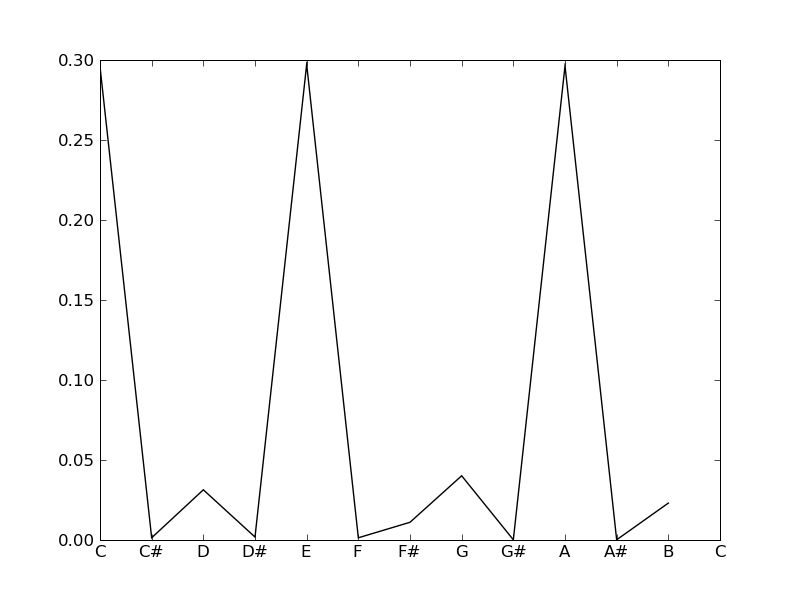
\includegraphics[width=7.5cm]{images/posteriors/posterior-profile-0_5.png} &
        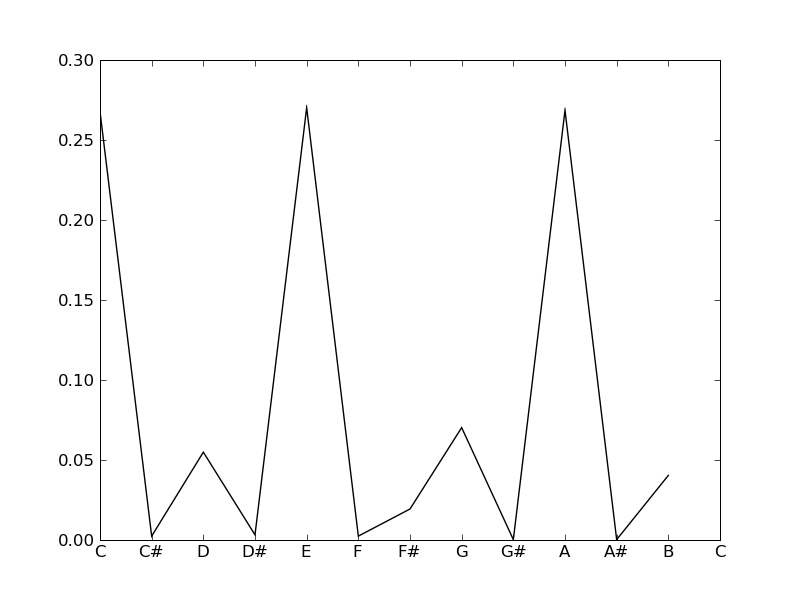
\includegraphics[width=7.5cm]{images/posteriors/posterior-profile-1.png} \\
        $\alpha=0.5$ & $\alpha=1$ \\
    %%	\vspace{1cm} & \\
        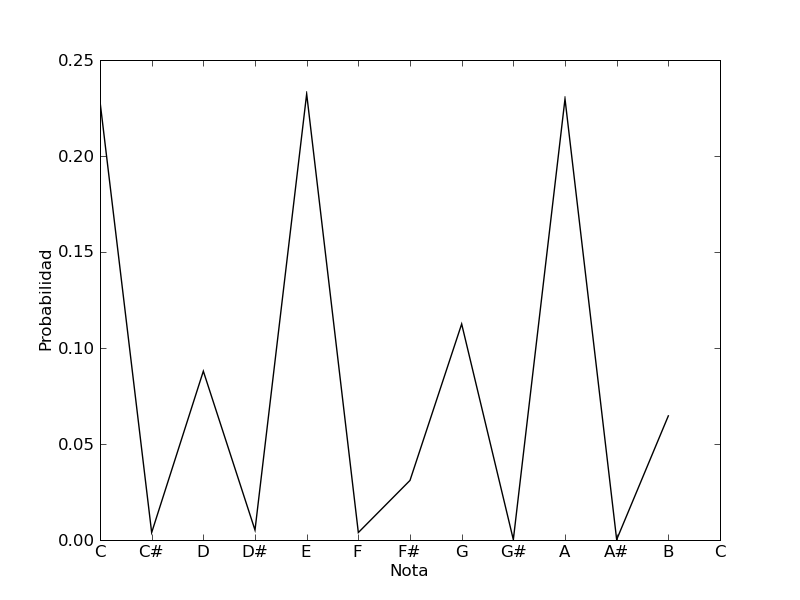
\includegraphics[width=7.5cm]{images/posteriors/posterior-profile-2.png} &
        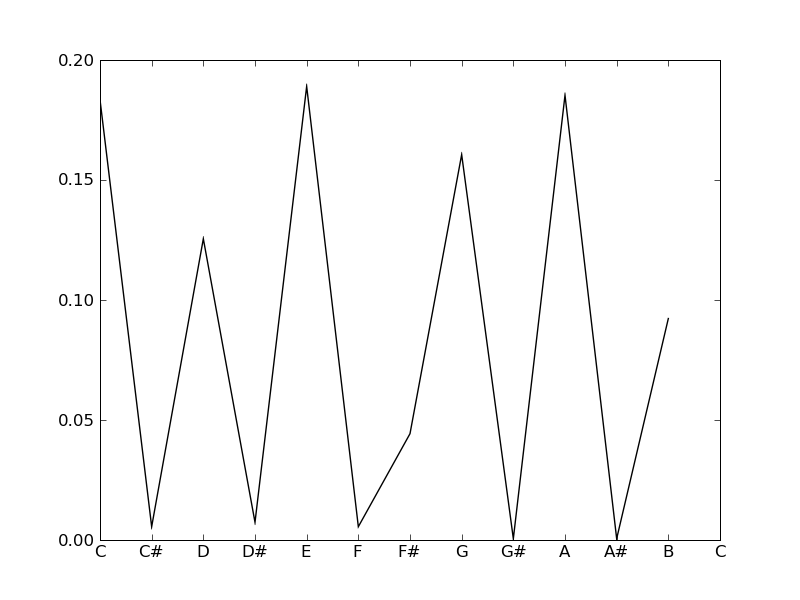
\includegraphics[width=7.5cm]{images/posteriors/posterior-profile-4.png} \\
        $\alpha=2$ & $\alpha=4$ \\
    %%	\vspace{1cm} & \\
        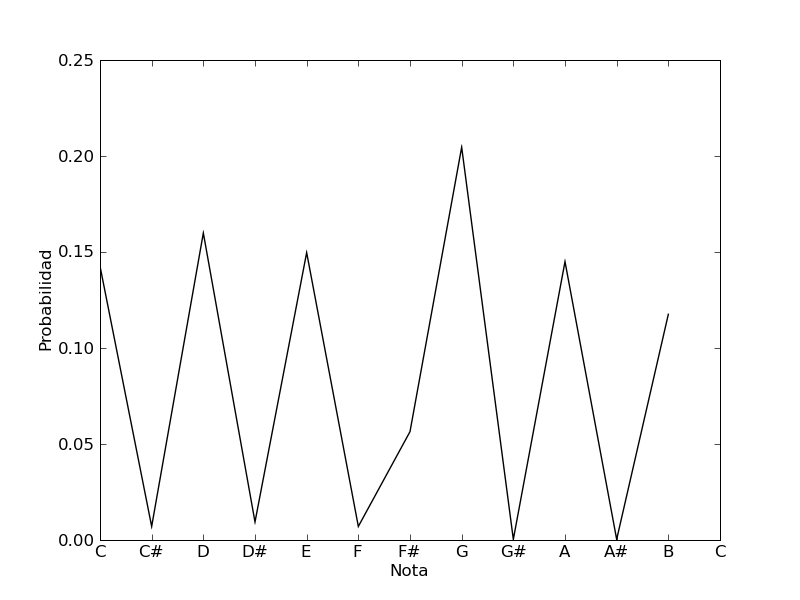
\includegraphics[width=7.5cm]{images/posteriors/posterior-profile-8.png} &
        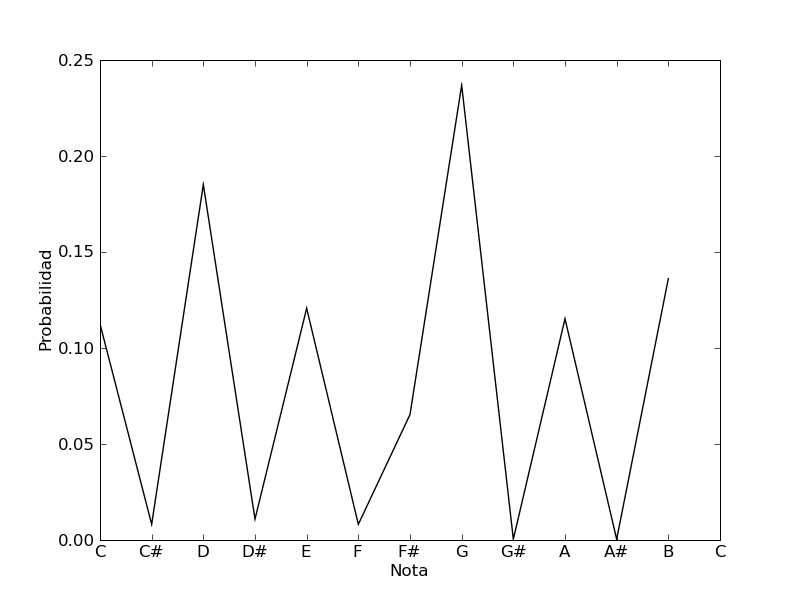
\includegraphics[width=7.5cm]{images/posteriors/posterior-profile-16.png} \\
        $\alpha=8$ & $\alpha=16$ \\
    %%	\vspace{1cm} & \\

        \end{tabular}
        \caption{Distribuciones a posteriori de un contexto arm\'onico para distintos valores de $\alpha$}
        \label{fig:pitch_posteriors}
    \end{center}      
\end{figure}

El modelo planteado en esta secci'on hace ciertas asunciones impl'icitas de las que se desea dar detalle. 
Si bien el pitch profile que Krumhansl propone como mecanismo para caracterizar la tonalidad en la que se encuentra una pieza es suficiente para este prop'osito, 
podr'ia no serlo para generar una melod'ia. Como primer variac'ion, en lugar de que la probabilidad de una nota sea la proporci'on de tiempo que esta son'o en el tiempo, 
se podr'ia construir una familia de distribuci'ones indexadas por duraci'on. 'Esta ser'ia otra forma de reflejar el hecho de que notas largas tienden a ser estables.

Otra caracter'istica que no es tenia en cuenta en este modelo es el acento m'etrico que recibe una cierta nota. Es sabido que en posiciones m'etricamente m'as fuertes
existen restricci'ones sobre la estabilidad de las notas que se pueden tocar all'i. Nuevamente, una soluci'on podr'ia ser tener una familia de distribuci'ones indexadas
por el acentro m'etrico. Esto mismo ocurre tambi'en con las notas que reciben un acento estructural, sin embargo en la secci'on \ref{sec:phrases} se dar'a una posible
soluci'on a este problema. 
